%===================================== CHAP 2 =================================

\chapter{Background}\label{chpt:background}

% Connectionism
\section{Connectionism and deep learning}
The processing unit in an artificial neural network (ANN) is the artificial neuron. This unit may be represented as a single activation value, symbolising a neuron's internal state. In order to process information, vectors of activation values representing neuronal activation in a layer may be multiplied with matrices of weights, representing connections between neurons of different layers, i.e. synapses and synaptic connection strengths. This linear algebra operation propagates information throughout the network, and is commonly known as the feed-forward process in the classical domain of neural networks. In order to arrive at a weight configuration which lets a network perform a certain task, it may be trained using gradient descent in weight-space \citep{Hinton1989}. A common implementation is by  back-propagating an error signal through the network whilst attempting to minimize it, adjusting the network weights accordingly. The error is usually a loss function such as the l2-norm (see appendix A) of the difference between an acquired output and a target output, which may be thought of as the Euclidean distance in space. This technique of training a neural network; back-propagation, was largely popularized by \cite{Rumelhart1986}. Furthermore, \cite{Rumelhart1986} made the important choice of electing the logistic function, also known as the sigmoidal function, as their candidate transfer function for propagating activation values through synapses in their experiments and models. That is, the sum of a neuron's input is run through the sigmoidal function, which has two important characteristics: \textbf{(1)} it puts a lower and upper bound on the activation values of a neuron, (-1, 1), and \textbf{(2)} it is continuous and differentiable, resulting in numeric methods of differentiation being applicable for weight adjustment relative to the change in activation values. In other words, the transfer function may be thought of as a crude mathematical approximation to a neuron's internal dynamics.
When ANNs are constructed in this manner; as simple activation values, weights between the values, and transfer functions between the different layers, the resulting models are often referred to as connectionist models. An example includes the aforementioned traditional feed-forward back-propagation (FFBP) neural networks of \citep{Rumelhart1986}.

% Other connectionist research here? Do I need further examples? Keith only mentioned that I should include and example from computational neuroscience. I feel that I should include some more stuff that condenses the context which I would like to establish for the model that I am actually investigating.
When it comes to deep learning, this is primarily an engineering discipline in the sense of its models being more focused on creating applicable systems and solutions, rather than on explaining the biological systems from which they originate. I would like to emphasize that despite this; it is the synthesis of neuroscience, psychology, and computer science that has given rise to the field of artificial neural networks \citep{McCulloch1943} and its various sub-fields. Furthermore, they continue to be factors in advancing the field's applications. This is exemplified by the recent deep learning algorithm in which the biologically inspired long short-term memory (LSTM) unit \citep{Hochreiter1997}, and the even more recently proposed, and perhaps simpler, gated recurrent unit (GRU) \citep{Mnih2015}, enables deep networks to capture temporal dependencies in data sets - adding a fundamental and crucial richness to what correlations and structures that may be captured by this class of general learning algorithms; namely long-term temporal dependencies within data.
While a unit such as the GRU does not necessarily demonstrate the workings of the biological brain, it does demonstrate that studying aspects which the biological brain captures, and translating them into algorithmic principles or requirements, may significantly improve engineered solutions, having both computer scientific value and impact. In other words; attaining further knowledge within the domain of computational neuroscience may lead to algorithmic advances within deep learning, and vice versa. Had the GRU been discovered first, this could have led to the hypothesizing of recurrence being crucial to capturing temporal dependencies within neural networks. Even though this is already a widely appreciated fact within neuroscience, the LSTM and GRU may still have an impact on the field of neuroscience, as we continue to discover why they enable algorithms to perform more sophisticated types of processing. While it is not the aim of this thesis to categorize algorithms as belonging to one branch or another within the associated fields of neural networks, it is my intent to outline connectionism and computational neuroscience in order to \textit{clarify} the synthesis of fields related to neural networks and AI, as well as to establish the context for the model which is studied in this thesis. A further review of computational models is included later in this chapter, after a foundational neuroscientific background has been visited.


% =================================================================================================
\section{Catastrophic forgetting}\label{chpt:catastrophic-forgetting}

Catastrophic forgetting \citep{McCloskey1989, Ratcliff1990} is as outlined in the introduction (chapter \ref{chpt:intro}); the forgetting of model parameters for a domain in which the model has previously been trained. This may occur to such an extent that the network performance is equal to that of random weight initialization.

\cite{McCloskey1989} were some of the first to analyse catastrophic interference, noting that it seems inevitable during sequential learning in connectionist models. Furthermore, they found that the cause for interference is that the newest weight adjustments reflect the newest information more heavily. In other words, old information is by the nature of the sequential learning disrupted by the correlations currently being extracted from the current pattern. This remains a fundamental issue for algorithms employing sequential learning, including algorithms such as back-propagation, and other gradient-based algorithms. In fact, it remains a central issue for all network-based algorithms which perform a type of sequential learning.

\cite{Ratcliff1990} studied forgetting in neural networks, and found similarly to McCloskey and Cohen that back-propagation networks are prone to catastrophic forgetting. Furthermore, he found that as more information is learnt by an FFBP ANN, its ability to discriminate between previously presented patterns and the ones currently being learnt is reduced. This contrasts empirical studies of biological neural networks \citep{Ratcliff1990}, and led \cite{Ratcliff1990} to propose a mechanism for reducing catastrophic forgetting in ANNs. Namely by using neurons which would selectively \textit{respond} to certain input, which he termed 'response nodes'. However, his proposed model only alleviated, and did not successfully eliminate the problem of catastrophic forgetting. Note that various attempts were made by both of the two aforementioned authors, \citep{McCloskey1989, Ratcliff1990}, none of whom attained a model which eliminates catastrophic forgetting in FFBP ANNs.
% French's node sharpening:
\cite{French1992} examined FFBP ANNs in a very similar context, attempting to eliminate catastrophic forgetting by implementing 'node sharpening'. Arguing that catastrophic interference occurs due to overlap in input patterns, \cite{French1992} suggested that the issue could be alleviated, or even resolved, by creating a non-overlapping memory. Therefore he reviewed previous research such as the ALCOVE algorithm \citep{Kruschke1992}, on using a sparse distributed memory, in which information would rarely overlap. He found this to alleviate catastrophic forgetting to a certain extent. However, it did so by implementing a very large address space. Once this address space would become digested, catastrophic forgetting would indeed still occur. It is worth noting that using a sparse distributed memory requires an algorithm to be able to construct hyperplanes in which the input data is successfully separated. This may result in less generalizability in the network model, if representations are distributed across distinct sub-networks due to the hyperplane mapping.
Node sharpening as proposed by \cite{French1992} locally constrains input patterns to enhance the most prominent input features, effectively resulting in sparse representations. This results in less "noise" being propagated throughout the network, the most principal input nodes being in focus, and a significant reduction in catastrophic forgetting. However, this is done at the cost of attaining a less generalisable model, as node sharpening only looks at the \textit{n} most prominent nodes. 

The aforementioned process of node sharpening is strikingly similar to using convolutional networks for feature extraction, which was one of the inventions that re-instated neural networks as the state-of-the-art within domains such as image classification \citep{LeCun2015}. It should be noted that today's solutions such as the seminal deep convolutional network of \cite{Krizhevsky2012} performs a much more rigorous analysis of the input vector before passing it to the subsequent layers of the network. Additionally, the method with which node sharpening is performed is a fairly biologically implausible algorithm, though feature extraction itself, e.g. extracting the most important features within a visual scene, is believed to occur biologically speaking. The mechanism with which this occurs is believed to be more similar to feature extraction using ConvNets, the convolution operation, however, being performed by the plastic neural network itself.

Today's state-of-the-art algorithms employ different transfer functions, network topologies, and neuron-models, when compared to French's (1992) node sharpening model. This may render the claim that a trade-off between catastrophic forgetting and generalisation is inevitable obsolete.
Building on French's (1992) former work, \cite{French1994} proposes a model which \textit{dynamically} sharpens the most relevant input nodes. Once two different outputs have been presented to a standard FFBP network, a context bias is calculated in the hidden layer, and propagated back to the input layer. Shortly put, this emphasizes the differences of the distinct categories, focusing on segmenting and orthogonalizing on the most prominent properties in differentiation. This results in more orthogonal, well distributed patterns being learnt.
Although this type of segmentation works well, it remains similar to the former approach of \cite{French1992}, and suffers from the same type of trade-off between remembering and generalisation. As in other FFBP networks performing gradient descent in weight space, the algorithm will only succeed to find the most principal components, scaling with how much information the network is able to store (mainly affected by its size). As a consequence, failing to attain a sufficient accuracy for a given task could be due to ignoring the detailed information present in the segmentation process. Furthermore, it may be the case that only finding the most principal correlations in a distribution does not reveal the distribution's true nature, failing to extract precise correlations and properties. This is at the very core of the sensitivity-stability dilemma \citep{Hebb1949}, i.e. the trade-off which occurs between the learning of new and disruption of old information. One way way of addressing this dilemma is by multi-network systems, which \cite{French1994} suggests in his conclusion. This may produce refined solutions and abstractions and more sophisticated pattern-associations, although seemingly less computationally efficient. In this thesis, the dual-network memory architecture \citep{McClelland1995} is the elected architecture for model construction and implementation, addressing catastrophic interference, and how short- and long-term memory may be implemented by the brain by implementing two network modules. The state-of-the-art of dual-network memory architectures is reviewed below in chapter \ref{chpt:existing-models}, after further background material from computational neuroscience has been presented.


% -> Computational Neuroscience
\section{Computational neuroscience}

At the other end of the scale of neural networks, used to study emergent behaviour, we have computational neuroscience. In this discipline, Hebbian learning is often seen as the elected learning mechanism, particularly when it comes to the modeling of short-term memory, as it is generally regarded to be fairly biologically realistic, and results in rapid convergence in the computational models (one-shot learning is possible, and sometimes occurs in the model which is outlined in chapter \ref{chpt:existing-models}). 
Another aspect which may regarded as more biologically realistic is the algorithm $k$-winners-take-all ($k$-WTA), where the plausibility arises from regarding it as implementing lateral inhibition. In biological networks, lateral inhibition may occur due to inhibitory neurons depressing the activation of other neurons \citep{Rolls1998chpt1}; thus the term long-term depression. As for $k$-WTA; the $k$-winners may be regarded as inhibiting the neighbouring neurons of the layer. Note that the algorithmic approach diverges from the biological in that lateral inhibition may be arbitrary, and for a fixed number of $k$ neurons in $k$-WTA, whereas the brain is not likely to implement such a hard firing rate threshold (number $k$). Furthermore, depending on the implementation, activation values may be fixed, and possibly binary in the algorithmic approach to lateral inhibition; $k$-WTA.

%\subsection{Background}
While it is assumed that the reader is familiar with neural networks within AI, it is not assumed that the reader has any prior knowledge within neuroscience. Therefore I will present an overview of the neuroscientific concepts used in this thesis, with the aim of sufficiently covering the neuroscientific background knowledge that is used.
\\

\begin{figure}
    \centering
    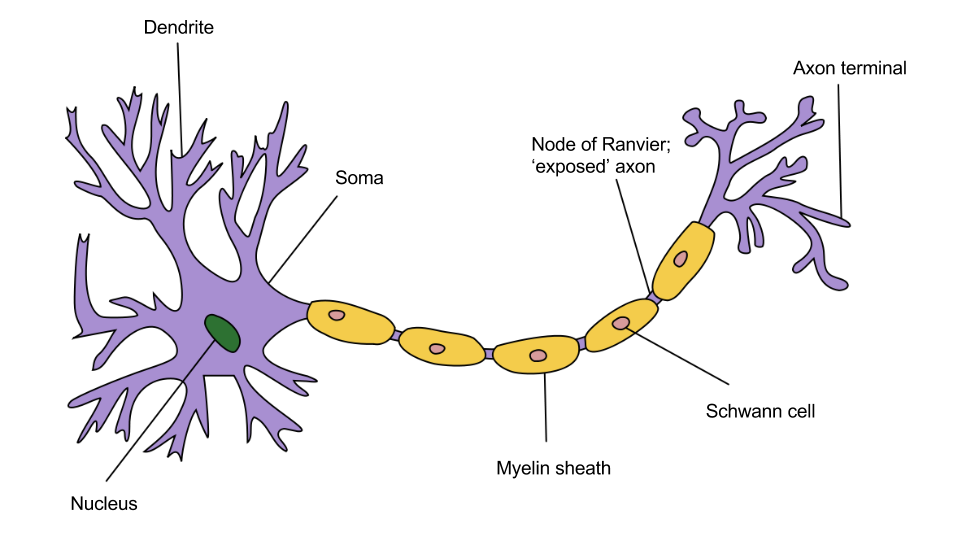
\includegraphics[width=12cm]{fig/neuron-figure-wikipedia}
    \caption{Illustrating a \textbf{neuron with its dendritic and axonal arborization}, i.e. branching. Please see figure \ref{fig:synaptic-cleft} for an illustration of a synaptic connection between a dendrite and an axon.
    The figure is adapted from Wikipedia: By Quasar Jarosz at English Wikipedia, CC BY-SA 3.0, https://commons.wikimedia.org/w/index.php?curid=7616130}
    \label{fig:neurons-synapses}
\end{figure}

% The very basics
As touched upon in the introduction, AI and neural networks borrows quite a bit of its vocabulary from neuroscience. Readers are very likely to encounter terms such as synapses, axons and dendrites when consulting the literature in computational neuroscience and other related disciplines. These terms refer to the connections between neurons, and the branches which physically enable them, respectively. A synapse actually consists of an axon, also referred to as a neuronal terminal, and a dendrite. Action potential may be propagated through an axon and its synaptic cleft to its connected dendrites, whose small branches are stretched out from other neurons' somata, or cell bodies - lying very closely to an axon terminal, and thus being referred to as connected (see figure \ref{fig:neurons-synapses}). When a neuron is intracellularly, i.e. internally, excited above a certain level, this triggers a response which results in the release of neurotransmitters, specific molecules, through its axon terminal. These neurotransmitters may then bind to the receptors (see figure \ref{fig:synaptic-cleft}), other molecular structures that bind to specific neurotransmitters, which are on the surface of the dendrite, triggering an intracellular response in the receiving neuron \citep{Campbell2015chpt9}.
Usually, neurons are multipolar, meaning that they consist of several dendrites, and one axon. While the dendrites branch continuously, the axonal arborization occurs at the axon terminal, i.e. the end of the axon, where it emerges from the myelin sheath; an isolating coating which enhances its conductance (see figure \ref{fig:neurons-synapses}). Note that there are periodically reoccurring gaps without myelin sheathing in figure \ref{fig:neurons-synapses}, called nodes of Ranvier \citep{Byrne2014chpt1p11}. These allow the absorption of ions through ion channels, which are thought to facilitate the action potential propagation coordination and timing \citep{Byrne2014chpt2p26}. This may also, however, perform a type of information exchange in interacting with extracellular ions. The Schwann cell is a type of support cell, which synthesizes myelin in the central nervous system \citep{Byrne2014chpt1p11}.
From this short outline of synaptic communication, it is possible to see how biological neuronal functioning potentially provides for a much richer type of information processing, when compared to the crude mathematical approximations that are used in most neural network models. Specifically, in the biological brain, different information may be carried by different types of neurotransmitters, triggering different intracellular responses, one of which may be altering the genome of the cell. Furthermore, a synapse may carry information at different speeds, depending on its structure, and synapses may be of different lengths, possibly carrying information not only at different paces, but also performing different intra-synaptical processing of the received relay molecules. Thus potentially performing a rich amount of information processing.

\begin{figure}
    \centering
    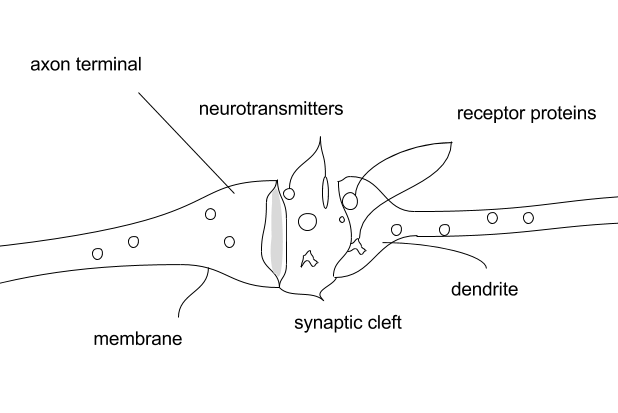
\includegraphics[width=12cm]{fig/synaptic-cleft}
    \caption{Illustrating \textbf{a synaptic cleft} in which two neurons are connected. Note that the axon of one of the neurons has released neurotransmitters, which may either excite or inhibit the receiving neuron after these neurotransmitters have bound to the receptors of its dendrite.}
    \label{fig:synaptic-cleft}
\end{figure}

I will regard emergent model aspects related to neuroscience and psychology through a connectionist lens; trying to keep what is biologically inspired biologically plausible where algorithmically feasible, and at the same time employing Ockham's razor \citep{Russell2009chpt18}. Both because the most simple hypothesis achieving the desired behaviour may be argued to be more likely, as it may potentially be more easily attained through evolution, but also because it is easier to implement, and provides for an axiomatic framework with basic building blocks, i.e. the researched algorithms. As argued by Hebb, the framework with which we study aspects of cognition has to be scientific. Therefore it has to be axiomatic, and deterministic in the sense of being algorithmically implementable. Furthermore, I argue that although approximations are made in artificial models, it may be possible to extract mechanisms, properties, and principles of biological neural network functioning. Upon extraction, these principles may be implemented and executed, studied, and perhaps even successful in capturing specific emergent aspects of cognition. I would like to emphasise that although a complete implementation of the biological knowledge we have of neural functioning is infeasible, it may be the case that algorithmic principles underlying the emergent neural functioning and neural network behaviour, may in fact be extracted. In this case, not only does it let us build a framework for studying neural networks - artificial and the like - it also lets do so using the scientific method, and Ockham's razor.

Some examples of computational models which have been able to model emergent neural functioning are models of spatial navigation in place fields and place cells \citep{OKeefe1976, OKeefe1996}, and the more recently discovered grid cells \citep{Hafting2005}.
Whether a mechanistic neuron-level understanding of the brain can be attained, and whether it encompasses what is required to have cognition emerge, remains another discussion. For as long as proven otherwise, the scientific method has to be employed, in which a testable framework needs to be used. We cannot but assume that aspects of cognition may be captured by a mechanistic neural level understanding of the brain.
For a further discussion on this topic, using examples from spatial navigation as those mentioned above to draw parallels from computational models to cognition, the interested reader may be referred to appendix E.

%\subsection{Computational Basis for Constructing Theories About Brain Function}
Propagation of action potentials may lead to synaptic modification in that dendritic branches grow closer to axon terminals, thus being more respondent to a connected neuron's release of neurotransmitters and activity. This process may be simplified and modeled as an activation value and function for the internal neuronal dynamics together with a weight symbolizing the synaptic connection strength. Various algorithms may be employed for synaptic weight modification in the computational model, as well as for adjusting neuronal activation values. These different approaches may be hybrids of primarily three neural network types as outlined by \cite{Rolls1998chpt1};
\textbf{(1)} conditioned stimulus with associatively modifiable synapses, i.e. Hebbian learning, or standard feed-forward back-propagation networks,
\textbf{(2)} purely recurrently connected associative networks, also known as Hopfield networks \citep{Hopfield1982}, and
\textbf{(3)} $k$-winners-take-all architectures, in which lateral inhibition is algorithmically simulated through letting the $k$ most active neurons fire, possibly with the remaining firing beneath a certain, low threshold. 
All of these approaches can be said to capture aspects of long-term potentiation in neural networks. However, the algorithm with which a network learns, i.e. how a network attains its weight-configuration, cannot be said to be biologically plausible in the case of minimizing an error signal through back-propagation. Hebbian learning, however, is more biologically realistic, as it updates its weights according to the firing activity between neurons, often representing firing rates. Interestingly, ANNs using Hebbian learning converge very quickly when compared to FFBP ANNs using gradient descent.

%\subsection{Hippocampus and Memory}
This thesis studies how memory may be implemented by the brain in an artificial and simplified neural network model. Below I review some of the material related to memory within the literature of computational neuroscience. More specifically, these theories are quite often based upon studies of the hippocampus.
Nearly half a century ago, \cite{Marr1971} argued that the hippocampus acts as a type of short-term or working memory, \citep{Rolls1998chpt6}. This has influenced later work, such as \citep{McClelland1995}, in proposing models where the hippocampus functions as an intermediary storage. The reasons for why the hippocampus has been hypothesized to constitute a type of working memory are multiple. One is that it is generally recognized that the hippocampus receives input from nearly every part of the brain, either directly or indirectly \citep{Rolls1998chpt1}, and so has the required input to integrate across different stimuli, or memories. Another is that the computational models of hippocampal operation, built upon the empirical data of its structure, i.e. topology and functioning, have been shown to have qualities that are well suited for performing essential operations that are related to memory and cognition.

Firstly, being able to quickly form new memories due to Hebbian learning is a crucial aspect for processing and remembering what happens during temporally constrained events. Therefore a mechanism for rapid learning needs to be present. As Hebbian learning performs weight adjustment according to the current firing pattern, this provides for a quickly converging learning mechanism in artificial neural networks. It is worth mentioning that one-shot learning is also made possible by Hebbian learning. 
When it comes to the potential storage capacity of memories in the hippocampus, there is a fairly large body of evidence suggesting that the hippocampus most likely employs a distributed type of encoding, resulting in that the capacity of \textit{patterns} which it may store is exponential to the number of neurons in a layer \citep{Rolls1998chpt6}. However, this does not imply that an exponential number of \textit{pattern associations} may be stored, i.e. an exponential number of different stimulus-response patterns, as this has been found to increase only linearly with the number of neurons in empirical studies \citep{Rolls1998chpt6}.

Secondly, integrating across memories by using an auto-associative network, which is thought to be constituted by the highly recurrent CA3-layer of the hippocampus, may in fact be part of what cognitively enables the brain to contextualize the self and the present.

Thirdly, very much related to the former point of being able to integrate across several sources due to the recurrent nature of CA3, a mechanism for implementing a form of episodic memory is essential in order to remember events, and to temporally associate different memories with one another. This is thought to be constituted by the CA3- and CA1-layers, where activity is both projected from the CA3 to CA1 through so-called Schaffer collaterals, and also recurrently to CA3. In other words, CA1 may then possibly temporally associate consecutive integrated memories that are relayed from CA3.

Fourthly, the hippocampus has been found to back-project its activity from CA1 to the EC \citep{Rolls1998chpt6}, and to the neocortex. The output from CA1 to neocortical areas may be hypothesised to perform a type of both recall, and memory consolidation. Recall in that the patterns may simply invoke activity given its output, and memory consolidation in that this activity, after having been processed by the hippocampus, may be stored in the neocortex. Addressing the latter, the neocortex has been found to perform significant long-term potentiation in its circuitry \citep{Rolls1998chpt6}. Such consolidation has also been hypothesized to occur primarily during sleep \citep{French2001}, in which a type of chaotic recall from a hippocampal network could produce pseudopatterns which may be learnt by the neocortex.
\\


% Outlined specifics of how the outlined hippocampal functions may be algorithmically attained and/or biologically occur AFTER presenting material on neural network computation in general?
It may now begin to become clear to the reader how certain aspects of hippocampal function may be algorithmically described, and thus how certain aspects of cognition may emerge from implemented models. Furthermore, these aspects may then be analyzed both from a connectionist perspective with regard to cognition, and also with regards to the information processing capabilities that the emerging phenomena gives or may give rise to. A short outline has now been presented on how hippocampal functionality is connected to psychology and neuroscience. I will proceed to connect these aspects to computational modeling and algorithmics below.

% Elaborate on $k$-WTA and connect it to feature detection/discovery (and self-organization)? Redundance reduction?
% Discuss orthogonalization in terms of simplification and losing out on information. Diluted connectivity?
% PCA bio. implausible, $k$-WTA more realistic.
One of the key components in the hippocampal neural processing as outlined by \cite{Hattori2014} in his model, is using $k$-WTA in the layer-wise processing. He notes that $k$-WTA seems to enable a much more sophisticated type of pattern-separation than ordinary transfer functions. This matches the observations and findings as outlined by \cite{Rolls1998chpt4, Rolls1998chpt6}. Namely that $k$-winners-take-all will reduce overlap in that only the $k$ most prominent units and neurons will dominate and inhibit the other neurons in a layer. Furthermore, they enable a more powerful separation of overlapping inputs. It should be emphasised that while $k$-WTA may resemble lateral inhibition, selecting an arbitrary value for the parameter $k$, quickly becomes biologically implausible. Therefore, computational models often rely on empirical studies of levels of activation within different brain regions in order to attain more realistic models. One example is the model which is outlined below, where \cite{Hattori2014}, building upon the work of \cite{Wakagi2008}, finds that selecting $k$ such that the layer-wise firing rate in his hippocampal module corresponds to the biologically observed firing rates, interestingly significantly improves the model performance compared to other $k$-values. I would like to emphasise that selecting only $k$ winners for a layer also leads to a quicker convergence and faster learning within the network, because weight updates are performed primarily by the $k$ winners relative to the current pattern. In a sense, less "noise" from the other neurons is present, and a more clear correlation and possibly pattern association is likely to be present for the network to extract. This may enable a network to reduce the redundance during feature or pattern correlation extraction, both functioning as an orthogonalizer quite similarly to principal components analysis (PCA), which extracts the most principal components of a data-set - only that $k$-WTA is more biologically realistic, and is able to perform a more separated type of extraction by activating different neurons.
Lastly, it is worth mentioning that while $k$-WTA may reduce overlap and separate inputs, it will also tend to result in similar patterns activating the same set of neurons. Therefore, $k$-WTA may also be regarded as pre-processing which will categorize patterns into categories of similar types, \citep{Rolls1998chpt1}. In other words, while $k$-WTA enables interesting information processing capabilities, the reader should bear in mind that this does not imply that the approach is not prone to some aspects of simplification due to orthogonalization - i.e. a type of diluted connectivity when using $k$-WTA due to reasons such as; too complex input data, sub-optimal convergence due to the initial random weight configuration, or simply basins of attraction being too close to one another, leading to divergence or spurious pattern extraction.

\begin{figure}
    \centering
    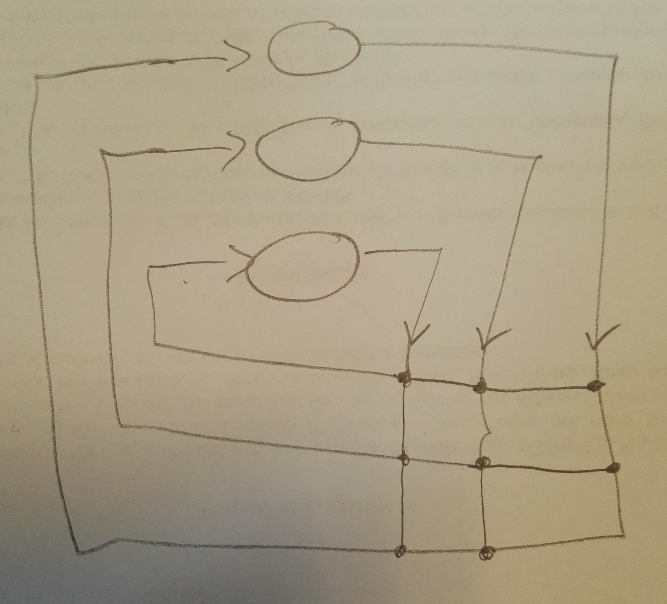
\includegraphics[width=8cm]{fig/hopfield-net.png}
    \caption{Illustrating a Hopfield net, which is \textbf{a simple auto-associative network}. Note that every neuron feeds into all other neurons of the network, which means that all information will be available to all neurons. Thus propagating it throughout the network until it reaches an equilibrium.}
    \label{fig:hopfield-net}
\end{figure}

% Elaborate on landscape for auto-associative nets? Mexican hat? Figure. Useful term: Topographical influence from closeness in input/feature space.
Another key aspect of computation previously outlined and present in the hippocampus, is auto-association and associative memory. Auto-association such as in a Hopfield network (see figure \ref{fig:hopfield-net}), associates one pattern with another very much like in a traditional network, only that the next activations are fed back into the very same layer, resulting in a mechanism for pattern completion. I.e. for only partial information of a previously learnt pattern, the values from the pattern will be propagated through previously learnt weights, which in turn reflect the pattern association previously learnt. This will most likely result in that the consecutive patterns will more closely resemble the learnt target pattern in the pattern association. This abstract outline of the process hopefully provides the reader with a gist about how auto-association enables recall through association of similar events and memories, as well as storage of these memories, and also why only a certain amount of memories may be stored in a short-term memory operating on these principles. This has been demonstrated in cases where an auto-associative network is taught two patterns that are too correlated. In that case, a simple Hopfield network will fail to perform pattern-completion, as it will be stuck between the two basins of attractions that are formed by the two different patterns \citep{Rolls1998chpt3}. This may be thought of as completing parts of for instance a pattern representing a letter, say 'a' - once part of the letter has been presented to the network; if another letter which is too similar, such as 'b' has been taught to the network, chances are that the Hopfield network then will push the network state towards both the 'a' and 'b' states at the same time. This may then lead to a new attractor state in which none of the letters is correctly recalled. Instead, it is likely that a combination of the two will be the result, or a cyclic pattern which cycles through hybrids of the two letters. There is a topographical influence from the closeness in the input or feature space.
In the general case, the possible state-space of an auto-associative network may be visualised as a 3-dimensional space, where the current input represents a point which moves in the space relative to gravity which is exerted on it in the space. Curvature in the space is then formed by training the network, which will result in areas curving downward towards an attractor point or state. Analogously, when such a point is created, its surroundings is necessarily also affected a bit by this spatial curvature, and will therefore alter its curvature, although slightly less, downward, giving a direction during traversal. From this analogy it may be seen that if two such points are created in each others' neighbourhood, there will be a given distance between them where the curvature exerted by the creation of both may form a new such basin. Additionally, if too many such points are created, the landscape may become impossible to traverse, or even pointing to one or very few basins - which may very well also be hybrids of previously learnt patterns, i.e. spuriously created patterns.
This brings us toward the importance of other qualities that are present in hippocampal models which largely removes these problems of redundancy and convergence in the CA3-layer.

\begin{figure}
    \centering
    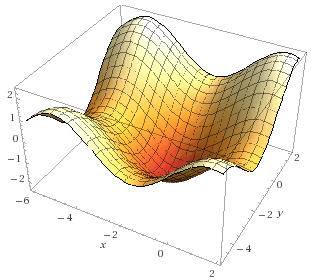
\includegraphics[width=8cm]{fig/simple-basin.png}
    \caption{\textbf{Illustrating a single basin of attraction}, the \textbf{axes representing the weight-space} which is traversed during learning and recall. Note that the further down into the basin one gets, the more likely the solution is to stay within the boundaries of converging towards the given solution (the red area of the basin).}
    % created using the simple formula: $f(x,y) = sin(x) + sin(y) + 0.5 sin(0.5 y)$.}
    \label{fig:simple-basin}
\end{figure}

% \begin{figure}
%     \centering
%     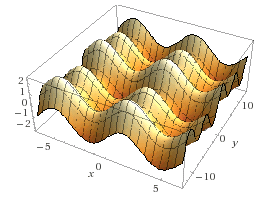
\includegraphics[width=8cm]{fig/whole-view-simple-basins.png}
%     \caption{Illustrating the basins of attraction of the entire weight space formed by the an auto-associative neural network. The illustration was created using the same formula as in figure \ref{fig:simple-basin}.}
%     \label{fig:basins-of-attraction}
% \end{figure}

While the classic XOR-problem is a matter of linear separability, solvable by the introduction of non-linear transfer functions in FFBP ANNs, issues are not quite as trivial in hippocampal models. When it comes to auto-associative memory, the forming of spurious basins of attraction (see figure \ref{fig:simple-basin}) in auto-associative networks may be addressed by qualities which are introduced by the hippocampus, and more specifically largely by the dentate granule cells of the dentate gyrus (DG), which project to cornu ammonis region 3 (CA3) (which is believed to constitute an auto-associative network in the HPC), both receiving projections from the entorhinal cortex (EC).

The dentate granule cells of the DG have been empirically observed in the rat hippocampus to be nearly approximately a sevenfold relative to the number of pyramidal cells which project to it from the entorhinal cortex \citep{Rolls1998chpt6}. Furthermore, while the firing rate of the EC has been observed to be about 10 \%, the firing rate of the dentage granule cells have been observed to be approximately 1 \% \citep{Rolls1998chpt6}.
Largely due to these facts, it is hypothesized that the role of these cells is to reduce overlap between and to separate overlapping inputs using inhibitory interneurons, i.e. $k$-WTA algorithmically speaking. Furthermore, the low contact between the dentate granule cells and the CA3-cells (i.e. low firing rate), referred to as expansion encoding \citep{Rolls1998chpt6}, also necessarily leads to a type of sparsification, in addition to further orthogonalization resulting from $k$-WTA in the expanded layer. Furthermore, it is believed that the dentate granule cells are strongly connected to the CA3-cells, which receive projections from EC, DG-cells, and recurrently from itself. This would then enable the DG-cells to strongly influence synaptic modification of the CA3-cells during learning, further enforcing new pattern correlations to be considered and possibly learnt \citep{Rolls1998chpt6}.

% Connect to DNMM.
% =================================================================================================
\section{Existing models}\label{chpt:existing-models}
% [May Need elaboration]

In their seminal paper, \cite{McClelland1995} propose a dual-network memory architecture in which the hippocampus is responsible for the consolidation of memories to the neocortex, with the neocortex storing semantic and episodic memory. The synthesis of recall from the deeper layers of the neocortex and representations in the working memory itself enables contexts to be distinguished or connected in the proposed model. The learning and consolidation to the neocortical module is essentially performed in an interleaved fashion; slowly potentiating and instantiating the memories from the hippocampal to the neocortical network. An approach closely resembling a bottom-up and top-down synthesis, where recall is combined with novel patterns. This raises the question of how such an interconnectedness is constituted both topologically speaking, as well as in terms of local information-processing. Furthermore, the question is whether principles from the environment of the neocortex and hippocampus need to be extracted and implemented to successfully have this functionality emerge in computational models, i.e. whether a synthesis of brain functionality constituted by additional parts would be crucial in regard to memory consolidation in the artificial model. For instance for the successful integration across memories. The proposed model of \citep{McClelland1995} suggests that the hippocampus and neocortex constitute the mechanisms for successful integration across memories, as well as keeping memories fairly intact. The specifics on how these mechanisms are constituted, however, remain obscure or undiscovered. This constitutes a core inspiration and foundation for the artificial neural network (ANN) model in this thesis. More specifically it lays out the foundation for investigating long-term memory and memory consolidation, by which I hope to attain more insight into mechanisms that enable generalizability and plasticity in ANN models.

The model of \cite{McClelland1995} largely ameliorates the problem of catastrophic forgetting in ANNs, outperforming other algorithms of the time by far. However, work on this model is fairly limited, and it is with the aim of further extending the architecture that I review implementations of it.

\cite{French1997} proposes a series of experiments that address the sensitivity-stability dilemma \citep{Hebb1949}, demonstrating that a pseudo-recurrent network model performs significantly better than traditional feed-forwad back-propagate networks, mainly inspired by \cite{McClelland1995}. Different experiments are used to illuminate several aspects of the pseudo-recurrent network model. The key finding is that pseudo-recurrent networks using pseudopatterns perform significantly better in terms of less catastrophic forgetting, suggesting that the brain may perform a type of pseudopattern compression and storage of information. Another point worth noting is that the networks that are simulated are of a fairly small scale, making them generalisable only to a certain extent due to network capacity. This seems to have been largely ignored by the authors. Therefore it would be interesting to look at the implications of both increasing the complexity as well as the scale of the network, such as in the models of \citep{Hattori2010, Hattori2014}. Note that the semi-distributedness of this paper's model arises naturally from the pseudo-recurrent neural network, as opposed to in the former papers of \cite{French1992, French1994}. This may suggest that the mechanism, which acts as an auto-associative memory, may also act as a predictor. In addition to completing incomplete, partial or fuzzy memories and retrieving them, it might therefore also provide a mechanism to filling in a story, or even imagining a story, creating it on the go by using the pseudo-recurrent mechanisms. This could suggest that the interleaving of memories in a pseudo-recurrent manner is at the heart of creativity, prediction and not the least; cognition. In relation to the thesis, I wish to investigate various successful or partly successful approaches for addressing convergence in the dual-network memory architecture. A key finding is that of pseudo-recurrence performing a crucial mechanism in interleaving and pattern generation. This may form a foundation for a comparative analysis in my future work, as well as providing insights into some underlying principles for the emergence of such mechanisms.

\cite{French2001} address the issues of the dual-network memory models in \citep{French1997, Ans1997}, illuminating key issues related to episodic memory, contextualisation, and pseudopattern generation and optimisation. In doing this, they conclude that the brain is likely to perform some kind of pseudopattern optimisation. Possibly in a stochastic way relative to how well it evaluates its performance and understanding of a currently perceived concept or state. When it comes to episodic memory, the work of \cite{Ans2000} is elaborated on by \cite{French2001}, in which only dissimilar pseudo-inputs were used for consolidation to a neocortical network. Results demonstrate that the model is capable of generalising to and thus learning all patterns (20 patterns, where only 13 are explicitly taught to the neocortical network). This strengthens the view that a dual-network memory model is crucial for successful integration across memories. Another aspect that is addressed in \citep{French2001} is contextualisation (in the dual-network memory architecture). \cite{Ans2000} demonstrate that their implementation of a dual-network memory model performs better using pseudopatterns with random initial input, rather than when retrieving more similar patterns from the neocortical module. This does pose an inconsistency both biologically and algorithmically speaking, because it is biologically implausible to retrieve an output representing the activity of the entire neocortical network, and algorithmically inefficient or possibly intractable with increasing network size, in order to interleave new memories with old. Furthermore, retrieving similar patterns mostly leads to a failure of convergence. This suggests that there may in fact be other, or more, principles that play a crucial role in the dual-network memory architecture. Summarising; the dual-network memory model offers significant benefits and advances in neural network models, but there seems to be an oversimplification related to pseudopattern formation and generation, affecting the integration across similar, yet separate memories. This is an aspect which I wish to further investigate in this thesis.
% Consolidation speed irrelevant - mechanism(s) for consolidation central \citep{French2001}.
It is also important to note that \cite{French2001} find that the pace at which memories are consolidated to a traditional ANN is of little relevance to the amount of information it may store - it is the mechanism with which the information is learnt that is of central importance in this regard. This makes the learning using pseudopatterns the central mechanism for increasing the storage capacity of the traditional ANNs.

\cite{Ans1997} address catastrophic interference in traditional backpropagation networks, demonstrating that it may be significantly reduced by using a pseudo-rehearsal mechanism \citep{Robins1995, Robins1996}. Such a mechanism is shown to be implementable by two reverberating neural networks, in which the first learns a certain pattern correlation, i.e. stimulus-response pair, after which the learnt pattern function is taught, or consolidated, to the second network by producing pseudopatterns - random input and corresponding output pairs; extracting the learnt pattern-mapping. Furthermore, in order to maintain previously learnt patterns in this traditional architecture, the way in which novel patterns are interleaved with old, is by consolidating the network configuration of the second network by pseudopatterns consisting of random input along with corresponding output, thought to represent the network configuration, to the first network. This results in that the first network considers both new information along with old. \cite{Ans1997} demonstrates that this does in fact significantly reduce catastrophic forgetting, and suggests that the brain may implement memory consolidation and interleaving in similar ways, although the mechanisms proposed by reverberation seems biologically unrealistic. Furthermore, they demonstrate that the same mechanism may be implemented by a slightly more realistic single-network model, in which the two networks are coupled to one single hidden layer, which then projects back to both input layers, thus enabling interleaving of new information with old, as well as re-injection of an extracted pattern. Note that this paper demonstrates a mechanism for transferring knowledge or information from one neural network to another, which one may argue is fairly realistic, given that biological neural networks tend to relay information to others. The idea of consolidating information is more closely studied in this thesis, and is also built upon by the architecture which is presented below.

\cite{Hattori2010} proposes a model which fundamentally differs from the former implementations of \cite{French1997, French2001}, and \cite{Ans1997} in that the hippocampal module is constituted by a chaotic neural network. Keep in mind that the phrases of hippocampal and neocortical networks should only be considered as borrowed terms for symbolising the networks of the model. The model networks are only very loosely coupled to biological functioning, with the approach outlined being only inspired by it.
\cite{Hattori2014} presents a novel ANN model based on his former work on the dual-memory architecture, where the short-term memory network is now a more complex and biologically plausible network; namely a simplified hippocampus model. \cite{Hattori2014} demonstrates in several experiments that catastrophic forgetting is reduced to a large extent in the new model, and furthermore that the model performance, in terms of recall rate and reducing catastrophic forgetting, is significantly improved relative to the dual-network memory models of \cite{Ans1997, French1997, Hattori2010}. \cite{Hattori2014} further demonstrates that the hippocampal network is capable of acquiring information rapidly, consolidating this to the neocortical network when it is successfully extracted in the hippocampal module.
However, the model is still not used to solve complex tasks, as the model is rather heavy in terms of computational complexity due to introducing more complex neuronal dynamics. The hippocampal network consists of McCulloch \& Pitts neurons, using the Oja rule for learning and updating connections between the different sub-modules, and less contrained Hebbian learning with forgetting in the recurrent CA3-connections. Please see below for further details on the model.
As for his experiments and results, he finds that mean goodness and perfect recall to be worse in the hetero-associative case when compared to the auto-associative for the model. This may suggest that a significant amount of plasticity is missing in the model. This is further supported by the observation that a much higher turnover-rate than observed biologically speaking has to be employed for tuning the model. Looking to complex systems theory, some noise or chaos is required to arrive at a phase-transition between regular and chaotic dynamics, i.e. the critical phase, in which learning is made possible and efficient, \cite{Langton1990, Newman2003}. By using a very high neuronal turnover in the model, this suggests that the high turnover rate could be what alleviates the lack of plasticity in the proposed model. Despite improving training performance and pattern extraction, using too high a turnover-rate may also introduce too much randomness, rendering the representations too coarse-grained. Therefore it would be interesting to see parameter adjustments for the hetero-associative case in the hippocampal module, as this may pose different constraints on the network. Particularly an analysis of the edge of chaos for the CA3-part is something which I wish to further investigate. Another important aspect would be attempting to temporally extend the model, in an attempt to capture how episodic memory may be constituted in a complementary memory model. Such a synthesis could potentially introduce novel aspects of high-level cognition.

\subsection{State-of-the-art}

\cite{Ans1997} demonstrated the important and interesting aspect of being able to increase a traditional FFBP ANN's storage capacity through embedding a learning algorithm using pseudopatterns in a dual-network architecture. More recently, \cite{Hattori2010, Hattori2014} demonstrates that a dual-network memory model which is more biologically plausible may in fact extract patterns in a more effective and biologically resemblant way, including one-shot learning, in an intermediary storage network. Thus having several qualities of short-term memory. Furthermore, his dual-network memory models show promising results in that they both outperform previous models of the architecture such as the models of \citep{French1997, Ans1997}, in classic sequential learning experiments for retroactive interference \citep{McCloskey1989}, where stimulus-response pairs of different training bases are learnt.
Hattori's (2014) model is reviewed and outlined below, and the methods and implementation used in this thesis is contained within chapter 3.

\subsubsection{The neocortical module}

\cite{Hattori2010} trains the neocortical module on the novel chaotically extracted patterns along with pseudopatterns. A set of pseudopatterns represents the current weight configuration of a network. In his paper, \cite{Hattori2010} employs two types of pseudopatterns, which he refers to as type I and II, in order to interleave the former weight configuration with the novel patterns it learns. Type I is constructed in a very simple way: A random input is presented to the neocortical network, and the output is retrieved. This is then stored as an input-output pattern, called a pseudopattern of type I.

Pseudopatterns of type II are constructed in a slightly different manner, the approach being as follows:

\begin{enumerate}
\item Retrieve an extracted pattern from the hippocampal network.
\item For each element of the pattern, reverse it with a probability $p_r$.
\item Present the pattern to the neocortical network, and store the retrieved input-output pair (pseudopattern II) in a set.
\item Repeat step 2. and 3. until a certain number of pseudopatterns of type II are obtained.
\end{enumerate}
Performing steps 1.-4. above results in a set of pseudopatterns of type II.

After pseudopatterns have been obtained, the neocortical network is simply trained on them along with the novel patterns extracted from the hippocampal network by chaotic recall, by using FFBP, i.e. standard gradient descent in weight space (as outlined in appendix A). Note that due to the nature of the pseudopatterns, old memories are actually interleaved with old. This may be seen by considering that pseudopattern I is in fact the output obtained by presenting a random input to the network, the output reflecting a compressed representation of the network weights at the time. When the network is trained on the pseudopattern along with a hippocampal pseudopattern, the algorithm of BP and gradient descent attempts to minimise the error between the old configuration of weights and the new hippocampal pseudopattern. Thus interleaving the old representation of memories with the new memory. In fact, \cite{Hattori2014} uses the exact same type of mechanisms for memory consolidation to the neocortical network.
Similarly, for a set of pseudopatterns II, as elements are reversed in the chaotically extracted pattern, the resulting pseudopatterns II reflect the old network configuration for distorted versions of the novel input patterns (for the current training set in the auto-associative scheme). This is a clever way of separating the old configurations from the new, as by creating slightly similar inputs, with outputs reflecting the former configuration the network will explicitly focus on these dissimilarities, and create separating hyperplanes for them. I.e. when training on the pseudopatterns II along with the new extracted patterns, it is ensured that the neocortical network has to minimise the loss between novel inputs and former \textit{similar}, yet separate inputs. Note that the only risk here is the case when the permutation of extracted pattern outputs by chaotic recall from the hippocampal network are permuted in a similar manner, which may possibly bias the neocortical network during training. This issue may be alleviated, or avoided altogether by training on several such pseudopatterns, which is part of \citeauthor{Hattori2014}'s (\citeyear{Hattori2014}) algorithm. Lastly, note that this is likely to be another factor resulting in the reduced goodness of fit for the hetero-associative patterns, other than the fact that the recall rate of the hippocampal module is lower. Namely that the hippocampal module \textit{output} is what is permuted and given to the neocortical network as \textit{input}. In the hetero-associative case, for it to have the same similarity to the extracted patterns as in the auto-associative case, it is the hippocampal pattern inputs which would have to be slightly permuted and given to the neocortical network in order to create pseudopatterns type II. This could be justified, and achieved, by means of bilateral neural network firing, i.e. firing from the output to the input, or simply relaying a distorted signal of the model input, biologically speaking.

Memory recall in the neocortical network may be performed by presenting input patterns to the neocortical network, and obtaining the resulting output from the network. Note that as outlined above, the neocortical network only learns using the pseudopatterns that are extracted by the hippocampal network. Therefore, some success criteria, such as perfect recall in the neocortical network, depends strongly on the perfect extraction rate of the hippocampal network (i.e. when all details of the pattern have been successfully learnt).

% ====================================
\subsubsection{The hippocampal module}
\subsubsection{\cite{Hattori2010}}
\begin{figure}
\centering
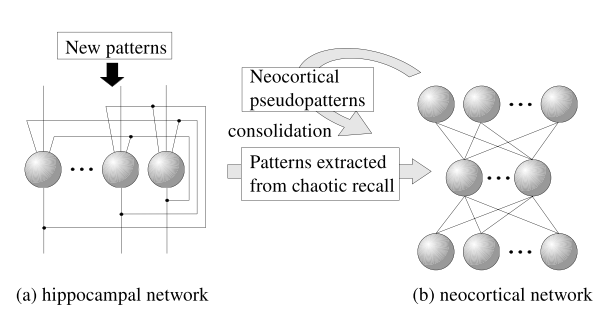
\includegraphics[width=11cm]{fig/hattori2010_model_structure}
\caption{Illustrating \textbf{\citeauthor{Hattori2010}'s (\citeyear{Hattori2010}) dual-network memory model}. (a) represents the hippocampal module, whereas (b) represents the neocortical module. Note that the hippocampal module implements a Hopfield network, from which seemingly chaotic behaviour emerges when combined with the neuronal dynamics. Adapted from Hattori, M. (2014). 'A biologically inspired dual-network memory model for reduction of catastrophic forgetting', \textit{Neurocomputing}, \textbf{134}: 262-268. Adapted with permission.}
\label{fig:hattori2010_model_structure}
\end{figure}

As may be seen in figure \ref{fig:hattori2010_model_structure}, \cite{Hattori2010} proposes a model in which the hippocampal (HPC) module is a single layer Hopfield network. However, the HPC module is not trained using gradient descent, but rather by Hebbian learning, which may be summarised as; fire together, wire together. Using Hebbian learning leads to faster convergence when compared to stochastic gradient descent \citep{Hattori2010}. Adopting \citeauthor{Hattori2010}'s (\citeyear{Hattori2010}) notation, the model may be formally outlined as follows, beginning with the equation for Hebbian learning;

\begin{equation}\label{hattori_hebbian_learning}
    \omega_{i,j}(t+1) = \gamma \omega_{i,j}(t) + x_i^{(k)} x_j^{(k)},
\end{equation}

where $\omega_{i,j}(t+1)$ is the weight between neurons $i$ and $j$ for time step $t+1$, $\gamma$ is a constant forgetting factor, $\gamma \in (0, 1)$, and $\textbf{x}^{(k)} = (x_1^{(k)}, x_2^{(k)}, ..., x_N^{(k)})$ is the $k$-th pattern that we want the network to learn. Note that $\textbf{x}^{(k)} \in \{-1,1\}^N$, which constrains $x_i^{(k)} x_j^{(k)} \in [-1,1] \implies \omega_{i,j} \in [-1-\gamma, 1+\gamma]$. $N$ is the number of nodes in the input patterns.

Further, \cite{Hattori2010} outlines the neuronal dynamics as follows,

\begin{equation}\label{hattori_next_output}
    x_j(t+1) = f\{\eta_j (t+1) + \zeta_j(t+1)\}
\end{equation}

\begin{equation}\label{hattori_eta}
    \eta_j(t+1) = k_m \eta_j(t) + \sum_{i=1}^{N} \omega_{i,j} x_i(t)
\end{equation}

\begin{equation}\label{hattori_zeta}
    \zeta_j(t+1) = k_r \zeta_j(t) - \alpha x_j(t) + a_j
\end{equation}

Adapted to the thesis notation, $u_j$ is neuron $j$'s activation value, where the value for the next time step is determined by two functions, namely $\eta(t+1)$ and $\zeta(t+1)$. Equation \ref{hattori_eta} takes into account its former input values through $\eta_j(t)$ for the current time step, in addition to summing over the inputs of its incoming synaptic connections. Equation \ref{hattori_zeta} includes a relationship to the neurons' previous activation values. Note that an external input parameter $a_j$ is also included in $\zeta_j(t+1)$, and that both equations \ref{hattori_eta} and \ref{hattori_zeta} have damping factors of refractoriness $k_m$ and $k_r$, respectively, discontinuing the impact of former function-values exponentially relative to the temporal distance. $f(u)$ is the sigmoid function as defined in equation \ref{sigmoid}, note however that a steepness parameter $\epsilon$ is also included, $\theta$ being divided by $\epsilon$ such that,

\begin{center}
\begin{math}
    f(\theta) = \frac{1}{1 + e^{\frac{-\theta}{\epsilon}}}
\end{math}
\end{center}

Introducing a Hopfield net as the hippocampal module lets the first network attain qualities of an auto-associative network, namely those similar to a short-term memory, or working memory. More specifically, it results in a content-addressable memory, along with the ability to perform perfect recall, unless the network's memory becomes digested as in the above general example (see the figures representing basins of attraction for an illustration of how this phenomenon may occur).
To some extent, a Hopfield net can be said to have a graceful degradation; i.e. its patterns are gradually distorted when the memory is diluted. It should be noted that this degradation is somewhat rapid in the case of a single-layer Hopfield network. In either case, this yields an interesting synthesis between the two networks, as the algorithm for memory consolidation does not have to reverberate the network configuration between two traditional neural networks that are trained using back-propagation. Instead, the associative network may be designed such that its parametrization lets it forget previous 'memories' at a pace such that it may learn up to a certain number of patterns, and thus consolidating the patterns as it learns. This is where algorithmic design of memory consolidation, i.e. learning in the second network, becomes of central importance. Note that the first network needs to be able to extract the patterns or memories that we wish to consolidate - but assuming that it does, it is the mechanism with which these are stored in the long-term memory network that is of central importance. This does not contrast previous models when it comes to the importance of interleaving old memories with new - it does however pose a significantly more biologically realistic model, as well as to open new opportunities for the short-term memory and pseudopattern generation. Pseudopattern generation is discussed further in the next chapter on the methods and implementation employed (chapter \ref{chpt:methods}).
% Outline differences from two reverberating FFBP ANNs.

% ====================================
\subsubsection{\cite{Hattori2014}}
\cite{Hattori2014} proposes a more biologically realistic dual-network memory model, based upon, and outperforming his former model. In the novel model, \cite{Hattori2014} proposes a significant architectural change in the hippocampal network, now modeling a more complex hippocampal network model, while the neocortical module remains the same. The hippocampal module consists of five layers, the three middle layers being inspired by different parts of the hippocampus; namely the entorhinal cortex, dentate gyrus, CA3, and two enclosing input and output layers. See figure \ref{fig:hattori_2014_model} for the topological structure of the novel model of \cite{Hattori2014}. 
Considering the neuroscientific background that is outlined above, the reasons for the significant performance increase can now be addressed by considering the different layers' algorithmic properties. 
Shortly put, the hippocampal module can be described as a competitive network, using $k$-WTA in all layers. Furthermore, sparsification results from partially connected layers, as well as from expansion encoding, i.e. a significant increase in the layer size relative to the preceding projecting layer, in the DG-layer. Note that the ratios between the DG-layer and the EC- and CA3-layer is the same as the ratios in the rat hippocampus, with the number of modeled neurons being about one thousandth. The relatively large DG-layer results in an expansion encoding, potentially recoding the neural activation values in the succeeding auto-associative layer of CA3, resulting in separated, yet initially similar patterns. It is worth mentioning that the DG model also implements neuronal turnover, which may further reduce overlap between inputs by re-instantiating some of the neurons' synaptic connections, contributing to the learning of separate new, yet similar patterns. Further model details are outlined below and in chapter \ref{chpt:methods}.

% The DNMM of \cite{Hattori2014} seems like a competitive network, having sparsification through in-EC and $k$-WTA, and to some extent orthogonalization from the DG-layer through expansion encoding, as well as neuronal turnover. (P. 54)

\begin{figure}
\centering
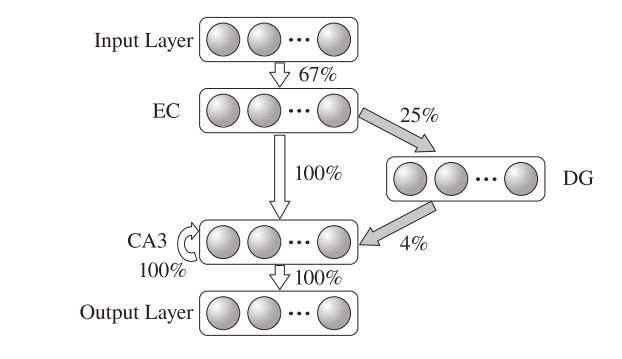
\includegraphics[width=10cm]{fig/hattori2014_hpc_module}
\caption{This figure illustrates \textbf{Hattori's (2014) proposed dual-network memory model}. Note that the EC is connected to both CA3 and DG, which in turn is also connected to CA3. The gray arrows are connections which are used solely during training.
Hattori, M. (2014). 'A biologically inspired dual-network memory model for reduction of catastrophic forgetting', \textit{Neurocomputing}, \textbf{134}: 262-268. Adapted with permission.}
\label{fig:hattori_2014_model}
\end{figure}

Note that in figure \ref{fig:hattori_2014_model}, the CA3-layer is fully connected both recurrently as well as to the output layer. As the EC-layer is connected somewhat sparsely to the DG-layer, and the DG-layer is very sparsely connected to the CA3-layer, this may constitute a form of compression mechanism as seen in auto-encoders. It is also worth noting that this poses a time-delay from when a certain input has been directly presented to the CA3-layer from the EC-layer, until the possibly compressed input arrives from the DG-layer. This might further constitute mechanisms similar to those of operating at multiple timescales, as well as mechanisms for abstraction.
It is worth mentioning that a slightly different transfer function is used by \cite{Hattori2014}. Namely,

\begin{center}
    $f(\theta) = tanh(\frac{\theta}{\epsilon})$,
\end{center}
where $\epsilon$ still is a steepness parameter.

Hebbian learning is still used as in equation \ref{hattori_hebbian_learning} for the CA3-layer and the CA3 to output-layer, relative to its former output;

\begin{center}
\begin{math}
    \omega_{i,j}(t+1) = \gamma \omega_{i,j}(t) + u_i u_j
\end{math}
\end{center}

However, between the EC and DG, EC and CA3, and DG and CA3 parts, Oja's rule is used (\cite{Hertz1991}, cited in \cite{Hattori2014}). Oja's learning rule is a modified type of Hebbian learning, restricting the weight space (to prevent divergence as a result of the chaotic behaviour). It may be formally outlined as follows,

\begin{equation}\label{ojas_rule}
    \omega_{i,j} = \omega_{i,j}(t) + \lambda u_j (u_i - u_j \omega_{i,j}(t)),
\end{equation}
where $\lambda$ is the learning rate for the Oja neurons. Note that the input and output layer neurons are bipolar ($\pm 1$), whereas the other neurons are binary. Every region is trained by a $k$-winners-take-all ($k$-WTA) approach, in which a fixed number of the $k$ most active neurons' activation values are propagated throughout the neurons' synapses. Neuronal activity is determined by firing frequency. Interestingly, \citep{Hattori2014} notes that the non-linear separation of $k$-WTA seems to be far more powerful than that of non-linear transfer functions. Furthermore, he notes that non-linear transfer functions may actually reduce the performance of $k$-WTA.

When it comes to the DG-layer of the model, it consists of 1600 artificial neurons, whereas the EC consists of 240, and the CA3 of 480. The input and output layers can be set to an arbitrary number of neurons, and are in most experiments set to 49 neurons each. Because of the ratio between the DG-layer and the EC-layer, the DG may perform expansion encoding. This may enable more intricate pattern correlations to be extracted by having a multiple number of neurons available for computation when compared to the layer which projects its output to the layer. Furthermore, it is believed that this constitutes a mechanism for decorrelating input patterns \citep{Rolls1998chpt2}, enabling the storage of similar, yet separate memories. Along with $k$-WTA, which biologically resembles lateral inhibition, it has been shown that including these mechanisms in a hippocampus-model increases the number of patterns that the model may store \citep{Wakagi2008, Hattori2014}. It is worth noting that while \cite{Hattori2014} employs the DG-layer in order to enable pattern decorrelation in the hippocampal module, this is only the case during learning, and the layer is not used during recall. The justification is that the DG is thought to function primarily as a pattern separator during learning. Biologically speaking, the DG is hypothesized to be able to strongly influence the synaptic modification in the CA3 during learning \citep{Rolls1998chpt6}.
One of the final keys to attaining a successful dual-network memory model is the introduction of neuronal turnover in the dentate gyrus. Neuronal turnover is the birth and extinction of a percentage $\beta \%$ of the neurons, here in the DG. Note, however, that while this is believed to occur to a very low degree biologically in the DG, a very high rate of $\beta = 50 \%$ is employed by \cite{Hattori2014}, with turnover after every training set. Possible reasons for this and associated implications, related to plasticity and convergence, is discussed earlier in this section, in that a high level of randomness, or noise, needs to be introduced in the artificial model, as it is less plastic due to mathematical approximations and model simplification relative to the biological system by which it is inspired. \cite{Hattori2014} demonstrates that input patterns become less similar when introducing neuronal turnover, which in turn drastically increases the number of patterns that may be stored in the HPC module. This demonstrates that neuronal turnover is a crucial mechanism for separation of similar patterns in the model, and possibly key to learning to distinguish between similar, yet separate memories and patterns.

Memory recall may be performed in the hippocampal network by chaotic recall after learning, i.e. presenting random input to the hippocampal model, waiting until it reaches some convergence criterion such as having a stable output for a number of time-steps, and considering the current input-output pattern as a 'chaotically' recalled memory, representing a learnt memory of the short-term memory model. 
% Elaborate on aspect of memory consolidation related to GABA either here, in the next subsection, or in the discussion.
% Principal cells biologically mostly excitatory; mutual inhibition implemented by inhibitory interneurons. (GABA)
Such a mechanism for pseudopattern extraction has been shown to create pseudopatterns that enable the neocortical network to extract the underlying function, i.e. mapping, of the pattern-association. It has further been hypothesized that a similar mechanism may be implemented by the brain \citep{French2001, Ans1997}. Note that \cite{French2001} found consolidation speed to be of no importance when it comes to retroactive network interference. Thus making learning through pseudopatterns the mechanism which itself enables the interleaving of several memories, as well as storage of them. This in turn makes the quality of the generated pseudopatterns a key key component in memory consolidation.
When it comes to the biologically implausible convergence criterion for when pseudopatterns should be generated, and memories consolidated, it may be hypothesized that when encountering a certain stability, the brain may release certain neurotransmitters that promote learning, such as glutamate, GABA, or dopamine, enabling memory consolidation. While remaining only a hypothesis, note that the algorithmic criterion for pseudopattern generation and memory consolidation is an aspect where the model diverges significantly from being the biological mechanisms from which the model is inspired.
Interestingly, when recalling previous memories in the HPC-model without using the DG-layer of the model, memories may yet be successfully distinguished. It seems that using the expansion encoding in the DG-layer together with $k$-WTA enables the model to extract the different properties in the similar pattern-associations. An observation which demonstrates that this mechanism is not sufficient, however, is the fact that hetero-associative patterns are not as easily extracted. The question remains whether they may still be as easily separated, only that the more complex function-mapping is more computationally heavy to extract.

% While using two reverberating neural networks that are trained using gradient descent remains biologically implausible and not that relevant for the current approach as outlined here, it is worth noting that a similar mechanism as described by \cite{French1997} for re-instantiating a previously learnt pattern to the hippocampal network if present in the neocortical network, would indeed be interesting as an alternative model for memory recall. An outline of how the hippocampus' operations may constitute memory is contained in the discussion in chapter \ref{chpt:discussion}.

To summarise, the outlined model of \cite{Hattori2014} introduces a novel hippocampal neural network model, inspired by hippocampal functioning. This results in a short-term memory network capable of acting as a working memory, having desired emergent qualities resembling those of the biological ones when it comes to; separation of overlapping, yet separate pattern-associations, integration across different memories (represented by different pattern-associations), quick convergence and the capability of one-shot learning, and the ability of extraction and perfect recall of low numbers of pattern-associations.
Note that the model is significantly simplified topologically speaking when it comes to the input and output connections. As outlined previously related to computational models and empirical studies on the hippocampus, the activity of CA3 is believed to be projected to CA1, which again relays the activity to cortical regions, as well as back to the entorhinal cortex \citep{Rolls1998chpt6}. This means that there is another layer which might be responsible for among others, two crucial aspects of hippocampal functioning. The first being episodic memory, in that the current memory is relayed back to the EC, and thus projected through the hippocampus and back to the CA3, possibly enabling relating consecutive memories and/or events to one another. The second being recall, and possibly memory consolidation, through back-projection to the neocortex after another synaptic information processing stage has been performed by projection to the CA1.
Thus leaving out CA1 in the hippocampal module results in that the model is incapable of episodic memory, i.e. relating consecutive memories, events or episodes to one another when temporally close. This is one of the limitations to the model that is studied. However, it does not imply that the underlying mechanisms for integrating across different stimuli and single pattern-associations, are not generalizable. Furthermore, even though back-projecting from a CA1-layer is not implemented, output is consolidated from an output layer, which is synaptically modifiable, and may thus be regarded as an approximation to the neocortical back-projections through which learning may occur. In other words, memory consolidation through pseudopattern generation and hippocampal module learning \textit{is} a very crude approximation to biological brain function and memory consolidation. Because of the interesting lines that may be drawn between neuroscience and psychology and the emergent model behaviour, I aspire to further study memory consolidation in the model of \cite{Hattori2014}, drawing parallels from the context which is established in this chapter.

Biologically, the experiment in \citep{Hattori2014, Hattori2010} is an adapted version of a classical learning experiment (\cite{Barnes1959}; cited in \cite{McCloskey1989}) created to test interference in connectionist models. \cite{McCloskey1989} address sequential learning in ANNs, and explore retroactive interference and possible links to this type of interference in connectionist networks by visiting the classical experiment of \citep{Barnes1959}, where lists, or sets of pattern-associations are learnt by subjects. Specifically, these experiments are meant to highlight retroactive interference occurring during sequential learning of different sets of pattern-associations. \cite{McCloskey1989} conclude that interference may be catastrophic in connectionist models when it is not in human subjects. However, as more recently addressed and outlined in chapter \ref{chpt:catastrophic-forgetting}; more biologically realistic models have been created within the paradigm, implementing memory in a dual-network fashion. So far, the comparative analysis has not been done with these models and the findings as outlined in \citep{McCloskey1989}, related to performance by human subjects, as models would have to implement more sophisticated autobiographical memory within these dual-network memory systems. I.e. the context is relevant to determining which pattern-association the current pattern should invoke (as is the case in the model of \cite{Hattori2014}). This could be simplified by regarding the context as part of the input-pattern - thus making the results attained in single-pattern-associations generalisable to a certain extent within this domain. Considering context as encoded in single pattern-associations remains a biologically implausible simplification, however, and the mechanisms for more complex types of memory remain unexplored in the domain of dual-network memory systems. I wish to perform a comparative analysis of the model of \cite{Hattori2014} and this thesis' implementation, drawing parallels to how the parametrization affects the quality of the attained pattern-associations, and the overall model performance. Furthermore, I wish to draw parallels between these relationships and the biological context addressed in among others \citep{McCloskey1989, Barnes1959}. This may give rise to hypotheses or suggestions for further experiments and discussions, as well as potential research spaces and future work.


% \section*{Notes}

% \subsection*{Information processing capabilities}

% Lateral inhibition

% $k$-WTA - separation, segmentation, etc.

% Interference conditions? Comparison with humans?

% \subsection*{Other}

% More on memory
% \\
% Possibility of using for instance 0.2 * sigmoid (in\_sum) for the neurons that do not fire 1?
% \\\\

% Approach topics that will be needed in the model and experiments.
% Concepts
% Terms
% Definitions
% Theory
% Memory. Working memory.
% The DNMA.
% This chapter is essentially: Terms, definitions, concepts, papers, contemplations, background theory. Revisit DNMA.
% Present previous model(s)
% Who is the reader..? A professor with general knowledge within AI
% \\

% \textbf{Notes from Rolls \& Treves:}

% Critic of HPC module as STM. Are these qualities transferable to networks in general? Principles? What do the experiments demonstrate?


\cleardoublepage